%==============================================================================
\chapter{Implementation and Use Cases}
\label{chapter:implementation_and_use_cases}
%==============================================================================
In this chapter we give a more detailed overview of the SANSA framework and the components developed during this thesis.
It also shows how they can be applied to various use cases.

In this chapter we address the following research question:

\begin{tcolorbox}
\textbf{RQ4}: How can we exploit large-scale \gls{RDF} datasets for a particular use case and ensure scalability?
\end{tcolorbox}

The chapter is organized as follows: First, in Section~\ref{sec:the-sansa-framework}, we give an overview of the SANSA framework, which contains the implementation of the methods presented in this thesis.
Later, we demonstrate the use of our components in a real use cases in Section~\ref{sec:alethio-use-case}.

This chapter is based on the following publications~\cite{lehmann-2017-sansa-iswc}
\begin{itemize}


   \item Danning Sui; \textbf{Gezim Sejdiu}; Damien Graux; and Jens Lehmann. "\href{https://gezimsejdiu.github.io/publications/sansa-hubs-and-authorities-transaction-semantics19-poster.pdf}{The Hubs and Authorities Transaction NetworkAnalysis using the SANSA framework}".  In 15th International Conference on Semantic Systems (SEMANTiCS), Poster \& Demos, 2019.
   
    \item Rajjat Dadwal; Damien Graux; \textbf{Gezim Sejdiu}; Hajira Jabeen; and Jens Lehmann. "\href{https://gezimsejdiu.github.io/publications/piping-clustering-eswc19-poster.pdf}{Clustering Pipelines of large RDF POI Data}" in Proceedings of 16th Extended Semantic Web Conference (ESWC), Poster \& Demos, 2019.
   
   \item Damien Graux; \textbf{Gezim Sejdiu}; Hajira Jabeen; Jens Lehmann; Danning Sui; Dominik Muhs; and Johannes Pfeffer, “\href{http://jens-lehmann.org/files/2018/semantics_ethereum_pd.pdf}{Profiting from Kitties on Ethereum: Leveraging Blockchain RDF with SANSA},” in 14th International Conference on Semantic Systems, Poster \& Demos, 2018.
  
    \item Jens Lehmann; \textbf{Gezim Sejdiu}; Lorenz Bühmann; Patrick Westphal; Claus Stadler; Ivan Ermilov; Simon Bin; Nilesh Chakraborty; Muhammad Saleem; Axel-Cyrille Ngomo Ngonga; and Hajira Jabeen, “\href{http://svn.aksw.org/papers/2017/ISWC_SANSA_SoftwareFramework/public.pdf}{Distributed Semantic Analytics using the SANSA Stack},”; in Proceedings of 16th International Semantic Web Conference - Resources Track (ISWC’2017), 2017.

    \item Ivan Ermilov; Jens Lehmann; \textbf{Gezim Sejdiu}; Lorenz Bühmann; Patrick Westphal; Claus Stadler; Simon Bin; Nilesh Chakraborty; Henning Petzka; Muhammad Saleem; Axel-Cyrille Ngomo Ngonga; and Hajira Jabeen, “\href{http://jens-lehmann.org/files/2017/iswc_pd_sansa.pdf}{The Tale of Sansa Spark},” in Proceedings of 16th International Semantic Web Conference, Poster \& Demos, 2017 ({\color{darkred}\textbf{Best Demo Award}}).

    \item Ivan Ermilov; Axel-Cyrille Ngonga Ngomo; Aad Versteden; Hajira Jabeen; \textbf{Gezim Sejdiu}; Giorgos Argyriou; Luigi Selmi; Jürgen Jakobitsch; and Jens Lehmann, “\href{https://svn.aksw.org/papers/2017/KESW_BDE_Workflow/public.pdf}{Managing Lifecycle of Big Data Applications},”; in KESW, 2017. \texttt{URL}:~\url{https://svn.aksw.org/papers/2017/KESW_BDE_Workflow/public.pdf}
    This article is a joint work with Ivan Ermilov, a PhD student at the University of Leipzig. 
    In this article, I helped on the implementation of the proposed approach and SC4 (Transport) use case, reviewed related work, and prepared of the experiments and analysis of the obtained results.

    \item Sören Auer; Simon Scerri; Aad Versteden; Erika Pauwels; Angelos Charalambidis; Stasinos Konstantopoulos; Jens Lehmann; Hajira Jabeen; Ivan Ermilov; \textbf{Gezim Sejdiu}; Andreas Ikonomopoulos; Spyros Andronopoulos; Mandy Vlachogiannis; Charalambos Pappas; Athanasios Davettas; Iraklis A. Klampanos; Efstathios Grigoropoulos; Vangelis Karkaletsis; Victor Boer; Ronald Siebes; Mohamed Nadjib Mami; Sergio Albani; Michele Lazzarini; Paulo Nunes; Emanuele Angiuli; Nikiforos Pittaras; George Giannakopoulos; Giorgos Argyriou; George Stamoulis; George Papadakis; Manolis Koubarakis; Pythagoras Karampiperis; Axel-Cyrille Ngonga Ngomo; and Maria-Esther Vidal, “\href{http://jens-lehmann.org/files/2017/icwe_bde.pdf}{The BigDataEurope Platform – Supporting the Variety Dimension of Big Data},” in 17th International Conference on Web Engineering (ICWE2017), 2017. \texttt{URL}:~\url{http://jens-lehmann.org/files/2017/icwe_bde.pdf}
    This article is a joint work with the BDE consortium. 
    In this article, I contributed within the semantic layer, more specifically; bringing the Big Data Analytics for RDF into BDE platform and co-contributing into dockerizing BDE components.
    
\end{itemize}


\section{The SANSA framework}
\label{sec:the-sansa-framework}
In this section, we introduce SANSA\furl{http://sansa-stack.net/}, an open-source\furl{https://github.com/SANSA-Stack} \emph{structured data processing engine} for performing distributed computation over large-scale \gls{RDF} datasets.
It provides data distribution, scalability, and fault tolerance for manipulating large RDF datasets, and facilitates analytics on the data at scale by making use of cluster-based big data processing engines.
It comes with: (i) specialised serialisation mechanisms and partitioning schemata for \gls{RDF}, using vertical partitioning strategies,
(ii) a scalable query engine for large RDF datasets and different distributed representation formats for \gls{RDF}, namely graphs, tables and tensors,
(iii) an adaptive reasoning engine which derives an efficient execution and evaluation plan from a given set of inference rules,
(iv) several distributed structured machine learning algorithms that can be applied on large-scale RDF data,
and (v) a framework with a unified API that aims to combine distributed in-memory computation technology with semantic technologies.

To achieve the goal of storing and manipulating large \gls{RDF} datasets, we leverage existing big data frameworks like Apache Spark\furl{http://spark.apache.org/} and Apache Flink\furl{http://flink.apache.org/}, which have matured over the years and offer a proven and reliable method for general-purpose processing of large-scale data.

\subsection{Architecture Overview}
\label{sec:sansa-architecture}

We now give an overview of SANSA framework.
Figure~\ref{fig:imp-use-cases-sansa-architecture} shows the overall architecture of SANSA that consists of four layers: \emphb{Knowledge Distribution \& Representation Layer}, \emphb{Query Layer}, \emphb{Inference Layer} and \emphb{Machine Learning Layer}.

\begin{figure*}
\centering 
	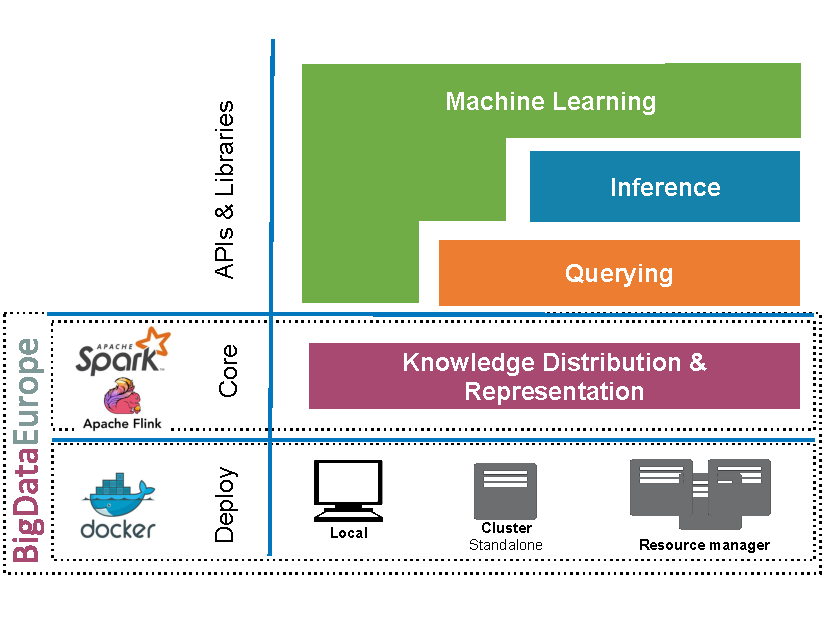
\includegraphics[width=0.95\columnwidth]{images/7_implemenation_and_usecases/sansa-architecture.pdf}
	\caption{\textbf{Overview of the SANSA stack}.
	The SANSA framework combines distributed analytics and semantic technologies into a scalable semantic analytics stack.}
	\label{fig:imp-use-cases-sansa-architecture}
\end{figure*}

In the following, we explain the role of each layer.

\defn{Knowledge Distribution \& Representation Layer}
It is the lowest layer on top of the existing distributed frameworks (Apache Spark or Apache Flink).
This layer mainly provides the facility to read and write native \gls{RDF} or \gls{OWL} data from \gls{HDFS} or a local drive and represent it in the native distributed data structures of the frameworks.

In addition, it also provides a dedicated serialization mechanism for faster I/O. 
SANSA aim to support Jena and \gls{OWL} \gls{API} interfaces for processing \gls{RDF} and \gls{OWL} data, respectively.
This particularly targets usability, as many users are already familiar with the corresponding libraries and thus would require less time to get productive with the SANSA stack.

Moreover, it allows users to compute \gls{RDF} statistics~\cite{sejdiu-2018-dist-lod-stats-iswc} and quality assessment~\cite{sejdiu-2019-sansa-dist-quality-assessment-iswc} in a distributed manner.


\defn{Query Layer}
Querying an \gls{RDF} graph is the primary method for searching, exploring, and extracting information from the underlying \gls{RDF} data.
\gls{SPARQL} is the \gls{W3C} standard for querying \gls{RDF} graphs.
Our aim is to have cross-representational transformations and partitioning strategies for efficient query answering. We are investigating the performance of different data structures (e.g., graphs, tables, tensors) in the context of different types of queries and workflows.
SANSA provides \gls{API}s for performing \gls{SPARQL} queries directly in Spark and Flink programs.
It also features a \gls{W3C} standard compliant HTTP \gls{SPARQL} endpoint server component for enabling externally querying the data that has been loaded using its \gls{API}s. These queries are eventually transformed into lower-level Spark/Flink programs executed on the Distribution \& Representation Layer.
At present, SANSA implements flexible triple-based partitioning strategies on top of \gls{RDF} (such as predicate tables with sub-partitioning by datatypes), which will be complemented with sub-graph based partitioning strategies.
In addition, it also support a so-called semantic-based query engine~\cite{sejdiu-2019-sansa-semantic-based-semantics} -- a scalable approach to evaluate \gls{SPARQL} queries over distributed \gls{RDF} datasets
Based on the partitioning and the SQL dialects supported by Spark and Flink, SANSA provides an infrastructure for the integration of existing SPARQL-to-SQL rewriting tools. 
This bears the potential advantage of leveraging the optimizers of both the rewriters as well as those of the underlying frameworks for SQL.
Currently, the Sparklify~\cite{2019-sansa-sparklify-iswc} implementation serves as the baseline.
It uses Sparqlify\furl{https://github.com/AKSW/Sparqlify} as a SPARQL-to-SQL rewriter for translating \gls{SPARQL} queries into Spark executable code.
Query results can then be further processed by other modules in the SANSA Framework.

\defn{Inference Layer} 
Both \gls{RDFS} and \gls{OWL} contain schema information in addition to links between different resources. 
This additional information and rules allows to perform reasoning on the knowledge bases in order to infer new knowledge and expanding the existing one. 
The core of the inference process is to continuously apply schema related rules on the input data to infer new facts. 
This process is helpful for deriving new knowledge and for detecting inconsistencies in the knowledge base.
It is well known that there is always a trade-off between expressiveness of a formal language and the efficiency of reasoning in that language. 
SANSA contains an adaptive rule engine that can use a given set of rules and derive an efficient execution plan from a given set of inference rules.

By using SANSA, applications will be able to fine tune the rules they require and -- in case of scalability problems -- adjust them accordingly.

\defn{Machine Learning Layer}
While most machine learning algorithms are based on processing simple features, the machine learning algorithms in SANSA exploit the graph structure and semantics of the background knowledge specified using the \gls{RDF} and \gls{OWL} standards. 
In many cases, this allows to obtain either more accurate or more human-understandable results.
There exist a wide range of machine learning algorithms for the structured data. 
However, the challenging task would be to distribute the data and to devise distributed versions of these algorithms to fully exploit the underlying frameworks. 
We are exploring different algorithms namely, tensor factorization, association rule mining, decision trees and clustering on structured data. 
The aim is to provide out-of-the-box algorithms to work with the structured data in a distributed, fault tolerant and resilient fashion.
Based on those advances, we will also be able to efficiently perform analytics to gain insights of the data for relevant trends, predictions or detection of anomalies.

\subsection{SANSA-Notebooks: Developer friendly access to SANSA}

SANSA provides Notebooks for an easy local deployment for development and demonstration purposes.
SANSA-Notebooks is an interactive toolkit on top of Hadoop-Spark-Workbench\furl{https://github.com/big-data-europe/docker-hadoop-spark-workbench} with Apache Zeppelin\furl{https://zeppelin.apache.org/}, which allows the copying of files from/to \gls{HDFS} and an interactive Spark code execution via a web GUI.
The architecture of SANSA-Notebooks is depicted in Figure~\ref{fig:notebooks_arch}.

\begin{figure*}
    \centering
    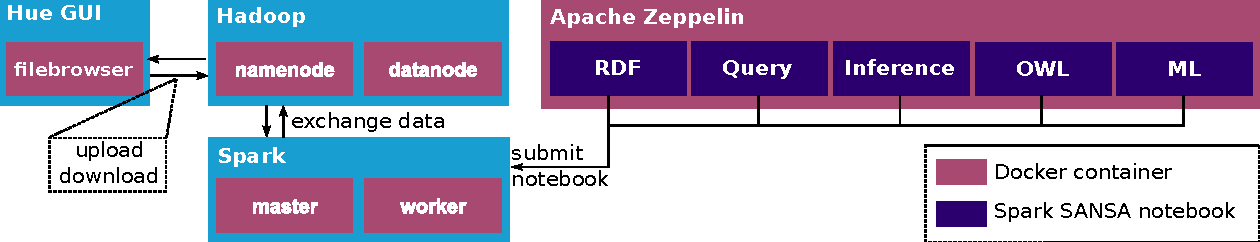
\includegraphics[width=\textwidth]{images/7_implemenation_and_usecases/SANSA-Notebook-architecture.pdf}
    \caption{\textbf{SANSA-Notebooks architecture}.
    An interactive toolkit on top of dockerized Hadoop-Spark-Workbench with Apache Zeppelin.}
    \label{fig:notebooks_arch}
\end{figure*}

We utilize SANSA-Notebooks (see~Figure~\ref{fig:notebooks}) in Big Data labs\furl{https://github.com/SmartDataAnalytics/MA-INF-4223-DBDA-Lab} and courses as they alleviate the complicated Hadoop/Spark setup and allow the students to focus on developing distributed algorithms on top of SANSA. 
Cluster deployment of the examples is also possible through Docker images (see SANSA-Examples Github repository\furl{https://github.com/SANSA-Stack/SANSA-Examples}). 
Additionally, SANSA is readily available from the Maven Central Repository. 
Thus it is straightforward to include it in other projects using Maven or SBT -- the most popular build managers for Scala -- for both Spark- and Flink-based setups. 

\begin{figure*}
    \centering
    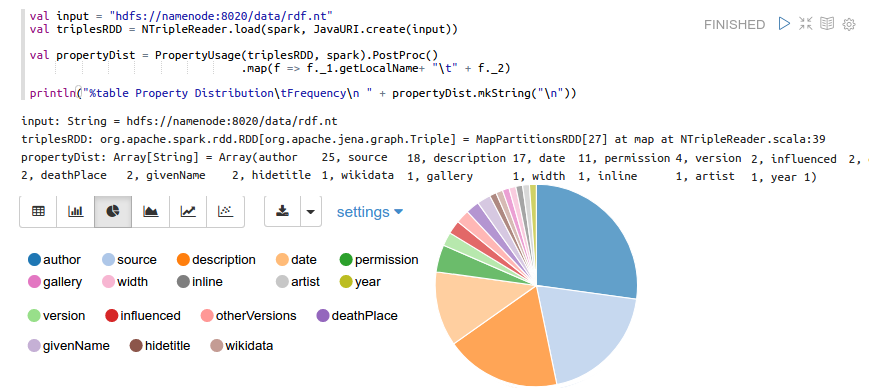
\includegraphics[width=.9\textwidth]{images/7_implemenation_and_usecases/RDF-Statistics_withoutlangTAG-cropped.png}
    \caption{\textbf{SANSA Notebooks example}.
    RDF-Stats Spark application running in SANSA-Notebooks with statistics visualization.}
    \label{fig:notebooks}
\end{figure*}

The notebooks present a compiled list of the SANSA examples\footnote{\scriptsize{The source code for all of them is provided at \url{https://github.com/SANSA-Stack/SANSA-Examples}}}.
These examples give a quick overview of the SANSA \gls{API}s.
SANSA is build on the concepts of distributed datasets (i.e \gls{RDD}, DataFrame, DataSet). 
A dataset is inferred from the external data, then parallel operations e.g. \textit{transformations} and \textit{actions} are applied which trigger a job execution on a cluster.
In the following, we provide a concise description for the examples grouped by the SANSA layers.

\begin{enumerate}
    \item \emphb{\gls{RDF}}.
    \begin{enumerate}
      \item Reading and writing triple files from \gls{HDFS} or file system and some basic triple operations.
      \item A distributed evaluation of numerous \gls{RDF} Dataset Statistics dubbed RDF-Stats (see~Figure~\ref{fig:notebooks}), for example, property distribution, class distribution, distinct subjects/objects/entities as well as statistics summary.
      \item A distributed evaluation of numerous \gls{RDF} Dataset quality assessment metrics i.e schema completeness, conciseness, interlinking, etc.
      \item Assigning weights to a given entity based on the Spark GraphX PageRank algorithm after triples have been transformed to a graph representation (i.e.~PageRank for resources).
    \end{enumerate}
    \item \emphb{Query}. 
    The example applies Sparqlify\furl{http://aksw.org/Projects/Sparqlify.html}, which is a SPARQL-to-SQL rewriter, for data partitioning and schema extraction. The queries are executed using the SparkSQL engine.
    \item \emphb{\gls{RDF} inference}. The examples apply a reasoning profile (\gls{RDFS} Full, \gls{RDFS} Simple, \gls{OWL} Horst, Transitive) on a given input file with an optimised execution plan.
    \item \emphb{OWL}. The examples provided for the OWL layer demonstrate the process of loading an \gls{OWL} file into Spark \gls{RDD}, a Spark Dataset, or a Flink DataSet.
    \item \emphb{Machine Learning}.
    \begin{enumerate}
        \item Clustering algorithms. Three examples for different clustering algorithms are provided, namely power iteration clustering, BorderFlow and modularity clustering. 
        They all take an \gls{RDF} graph as input and return the list of triples for each of the different clusters.
        \item Rule mining. This example applies association rule mining on a given RDF knowledge base. The output is the set of closed Horn rules that satisfy a support-confidence threshold.
    \end{enumerate}
\end{enumerate}

One of the powerful features of the SANSA Notebooks is that you can view the result set of the previous session within the Spark framework and, in case you have found some insight for your data and would like to share, you can easily create a report and either print or send it.


The main goal of the SANSA framework is to build a generic stack which can work with large amounts of linked data, offering algorithms for scalable, i.e.~horizontally distributed, semantic data analysis.
To validate this, we have developed use case implementations in several domains and projects.
   
A more detailed list of use cases with technical details and implementation is given on the following sections (cf. Section~\ref{sec:alethio-use-case}, \ref{sec:bde-use-case}, and \ref{sec:slipo-use-case}).

\section{Leveraging Blockchain RDF Data using the SANSA framework}
\label{sec:alethio-use-case}
With the hype on blockchain technologies and in particular in the Ethereum blockchain~\cite{wood2014ethereum}, many participants wanted to know more about the most impactful players across the blockchains transaction network.
In parallel, as the number of statements, actions and transactions in the network are increasing quickly, many ``Big Data'' challenges arise.
First, transactions are raw data and one cannot take advantage of them for further analysis.
To do so, Alethio designed EthOn (The Ethereum Ontology)~\cite{pfeffer2016ethon} which models such raw data as triples using the \gls{RDF} standard.
This ontology describes all Ethereum terms including blocks, transactions, contract messages, event logs etc., as well as their relationships.
Afterword, performing querying and analysis on such large-scale \gls{RDF} datasets is computing intensive.
To overcome these challenges, we have explored the potential of the SANSA~\cite{lehmann-2017-sansa-iswc} framework.
With SANSA on Spark, \gls{RDF} triples are loaded into Spark distributed and resilient data structured, namely the data frames, for further analysis.

\subsection{The Hubs and Authorities Transaction Network Analysis}
\label{sec:the-hub-and-authorities-use-case}
In this work, we perform an analysis (using well-known graph processing algorithms) of the value transaction network graph with the main focus on the Hubs and Authorities behaviors.
``Authorities'' are accounts who pay out to a large crowd of addresses, with high volume; while ``Hubs'' are entities who receive extensive \gls{ETH} flow into their accounts.
In this study, we do not differentiate these two roles but rank them all together as the biggest players/entities.

\subsubsection{Finding big Ethereum players with SANSA}
The Ethereum network graph contains nodes of external accounts which have had a transaction on the Ethereum blockchain.
The connection (edges) between such nodes on the network indicate the transaction relationship between them; when a node (an external account) sends \gls{ETH} to another, a transaction record is written, and an edge between them is added in the network with the direction of the \gls{ETH} flow. When we encounter multiple edges between same pairs of nodes, we summarize the edges as a single one\footnote{This optimization is also convenient practically as it is easier not to have duplicated edges in a graph.}. The edge weight is the total transaction value in Ether.
As an example, if address \emph{A} sends \emph{x} \gls{ETH} to address \emph{B} in total, there will be an edge of weight \emph{x} from node \emph{A} to node \emph{B}. 
In this study, self-loops i.e. transactions from an address to itself are omitted.

\begin{figure*}
\centering
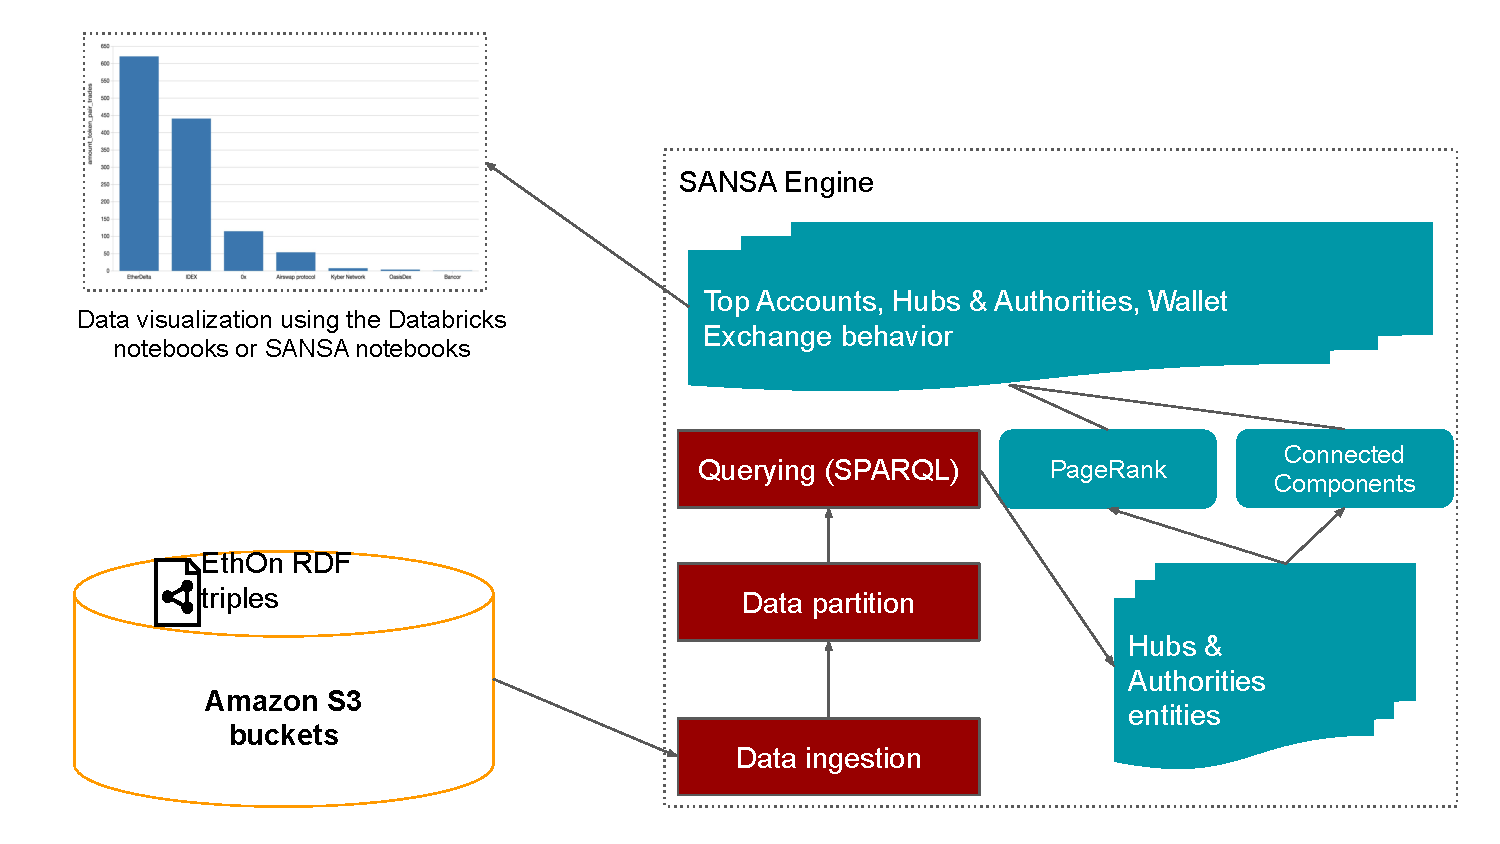
\includegraphics[width=1.0\columnwidth]{images/7_implemenation_and_usecases/hub-and-authorities-system-architecture.pdf}
\caption{\textbf{Hubs and Authorities analysis workflow}.
The architecture overview for gaining insight about Hubs and Authorities using the SANSA framework.}
% source: https://docs.google.com/presentation/d/1AoIvsI12ayLPFOqQlWkTk4rDG4GolY3YLs3yTql8lPg
\label{fig:hub-and-authorities-system-architecture}
\end{figure*}

SANSA framework has been used for efficient reading and querying of \gls{RDF} datasets using \gls{SPARQL} as depicted on Figure~\ref{fig:hub-and-authorities-system-architecture}. 
First, the data need to be loaded on an efficient storage that SANSA can read from. 
For that purpose, we use Amazon S3 buckets containing the whole \gls{RDF} Ethereum network transactions.
Afterword, SANSA data representation layer loads the data in a form of \gls{RDD} of triples. 
During this process, SANSA performs a data partition for fast processing and then aggregate and filter the data using the its query layer. Further, we applied two classic graph analysis algorithms via Apache GraphX: Connected Components and Page Rank.
Connected Components algorithm enables us to find the largest cluster of connected nodes, regardless of transaction direction. Within this largest cluster, we can derive the page rank score of all nodes. Top-ranked entities and their relation are visualized.

\subsubsection{Results}

\defn{Datasets}
The Ethereum dataset in the format of \gls{RDF} contains more than 17B triples.
For the sake of the experiment, we limited the dataset to 10,000 blocks which contain around 38M triples, including both value transactions and contract messages.

\defn{Top Accounts Analysis}
The PageRank algorithm was run over the largest connected component of 185,741 nodes (accounts) and 250,637 edges (aggregated transaction relations).

Figure \ref{fig:pagerank-score-distribution-of-top-50-accounts} plots the top 50 account's distribution. 
Based on the findings, we can see that these accounts are grouped on two different types: mining pool wallets, and (mostly centralized) exchange wallets. 

Figure \ref{fig:category-distribution-of-top-50-accounts} shows that 58\% of the addresses are controlled by exchanges, while another 12\% with convincing tags related to the mining pools.
The exchange and mining pool wallets can be found in the top position of our ranking, underlining the effectiveness of PageRank: Addresses related to mining pools allocate extensive amounts of payouts to their subscribed miners, resulting in large out-degrees, as well as high accumulated transaction value.
We can see that the main wallets are centralized exchanges which distribute (and receive) large volumes of the transaction to (and from) their deposit wallets, token contracts, etc.


\begin{figure*}[t]
 \begin{minipage}[b]{.5\textwidth}
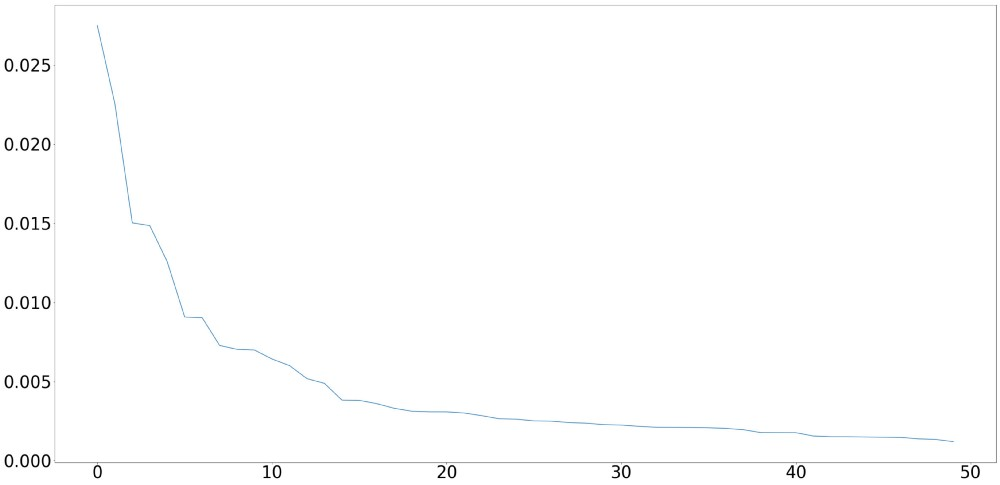
\includegraphics[width=1\columnwidth]{images/7_implemenation_and_usecases/pagerank-score-distribution-of-top-50-accounts.jpeg}
\caption{\textbf{PageRank Score Distribution of Top-50 Accounts}.}
\label{fig:pagerank-score-distribution-of-top-50-accounts}
 \end{minipage}
 \begin{minipage}[b]{.5\textwidth}
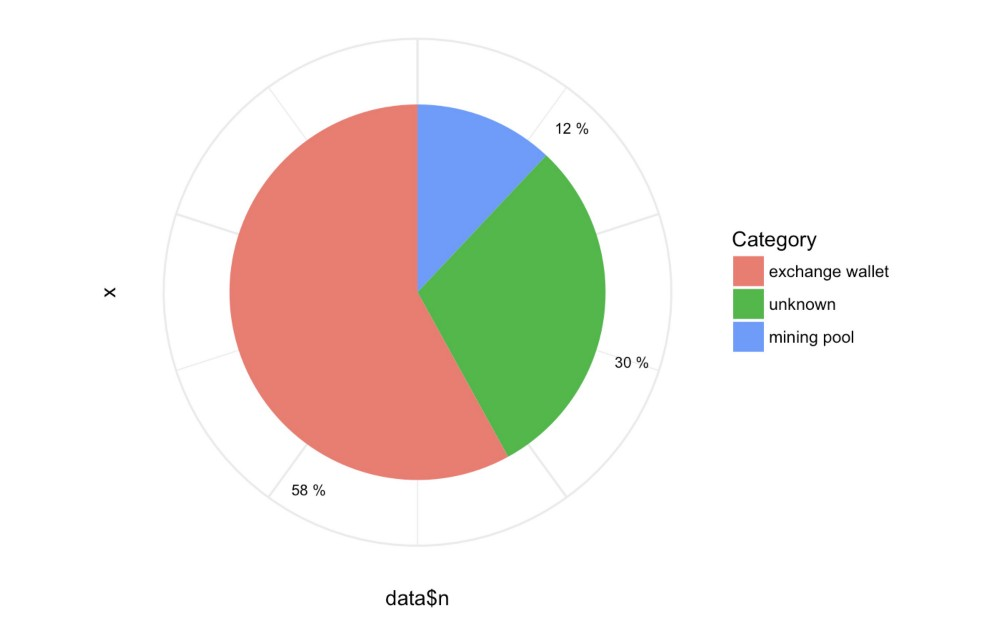
\includegraphics[width=1.0\columnwidth]{images/7_implemenation_and_usecases/category-distribution-of-top-50-accounts.jpeg}
\caption{\textbf{Category Distribution of Top-50 Accounts}.}
\label{fig:category-distribution-of-top-50-accounts}
 \end{minipage}
\end{figure*}

Our PageRank implementation successfully detects the most influential accounts across the network, corresponding to the Hubs and Authorities, connecting various transactors and carrying heavy flow weights.

\begin{figure*}[t]
\centering
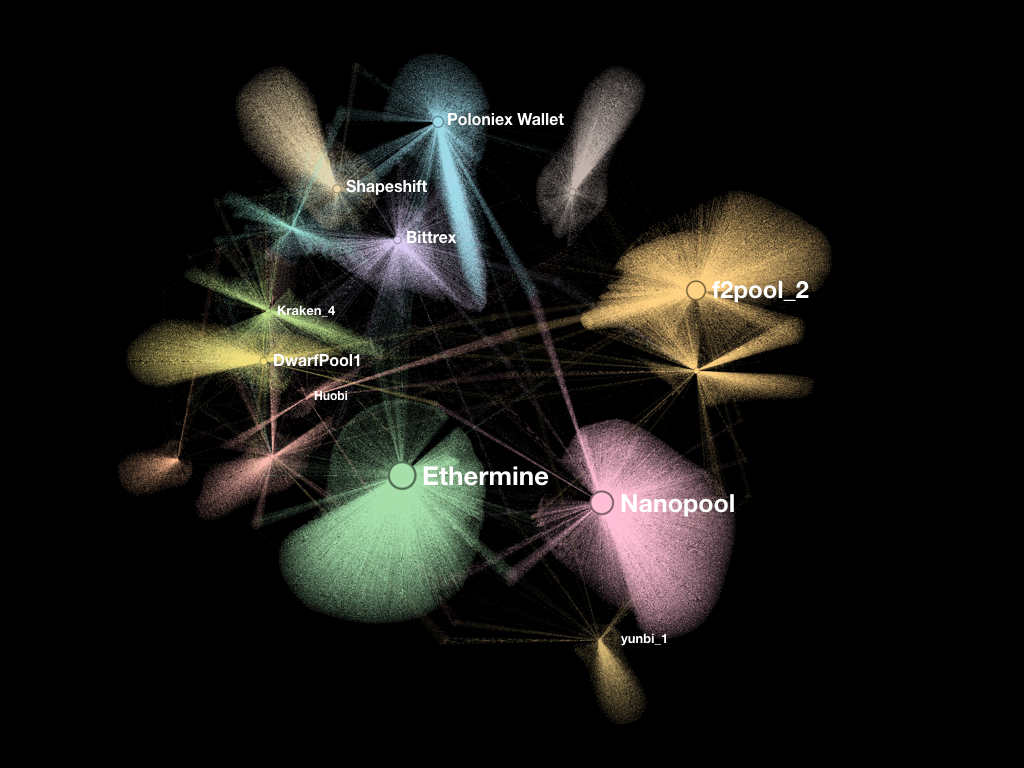
\includegraphics[width=1.0\textwidth]{images/7_implemenation_and_usecases/pagerank.jpeg}
\caption{\textbf{Transaction Network of Top Hubs and Authorities}.}
\label{fig:page-rank}
\end{figure*}

Focusing on those known accounts (with labels from Etherscan\furl{https://etherscan.io/}), we present (see Figure \ref{fig:page-rank}) the network overview of top hubs and authorities with transactions as edges surrounding them.

\defn{Typical Behavior Patterns of Exchanges' Deposit Wallets}
We investigated the associated transaction behavior of the exchange wallets.
Based on our finding, these behaviors can be grouped into three categories:
\begin{enumerate}
    \item \textit{Frequently paying out to certain exchanges' main wallets with a fixed, large value} -- From the scatter plot, the payout amount is always around a same value.
    \item \textit{Frequently receiving funds from the same exchange main wallets, and paying out to various token contracts} -- This is due to the activity which is associated with exchanges as they use external accounts as deposit addresses for collecting tokens based on trading needs.

    \item \textit{Frequently receiving funds from a group of ``miner'' accounts, with ``proxy'' accounts in between, which clean out their received \gls{ETH} within a short time frame} -- Usually, these addresses receive funds from miner accounts, which again get paid reasonable amounts by known mining pools, which we assume are mining rewards (usually around 0.11-0.12 \gls{ETH}).
\end{enumerate}

Despite pointing out the three typical behaviors above, they are not necessarily mutually exclusive.
There are addresses which share more than one of the deducted patterns.
These behavior patterns explored here are based on the labels we have gathered, and this may be different for other use cases.


\subsection{Profiting from Kitties on Ethereum}
\label{sec:kitties-use-case}

The Ethereum ecosystem generates a large amount of data, including but not limited to protocol-level data (e.g. average block time, gas prices), as well as application-level data (e.g. account interactions, smart contract deployments). 
To efficiently handle this volume of data, Alethio has investigated different tools and frameworks with one focus: the infrastructure should be resilient, load-bearing, and most importantly, scalable.
And so, for that reason to overcome the variety of the different data sources, Alethio introduces semantification of Ethereum network and uses SANSA as an underlying engine for large scale distributed \gls{RDF} based querying, reasoning, and machine learning on top of these \gls{RDF} datasets.
To show the joint effort between SANSA and Alethio, we describe a use case on how SANSA can be used to analyze Ethereum at new scales, as depicted in Figure \ref{fig:crypto-sansa}. 

\begin{figure*}[t]
\begin{subfigure}[b]{0.95\textwidth}
\centering
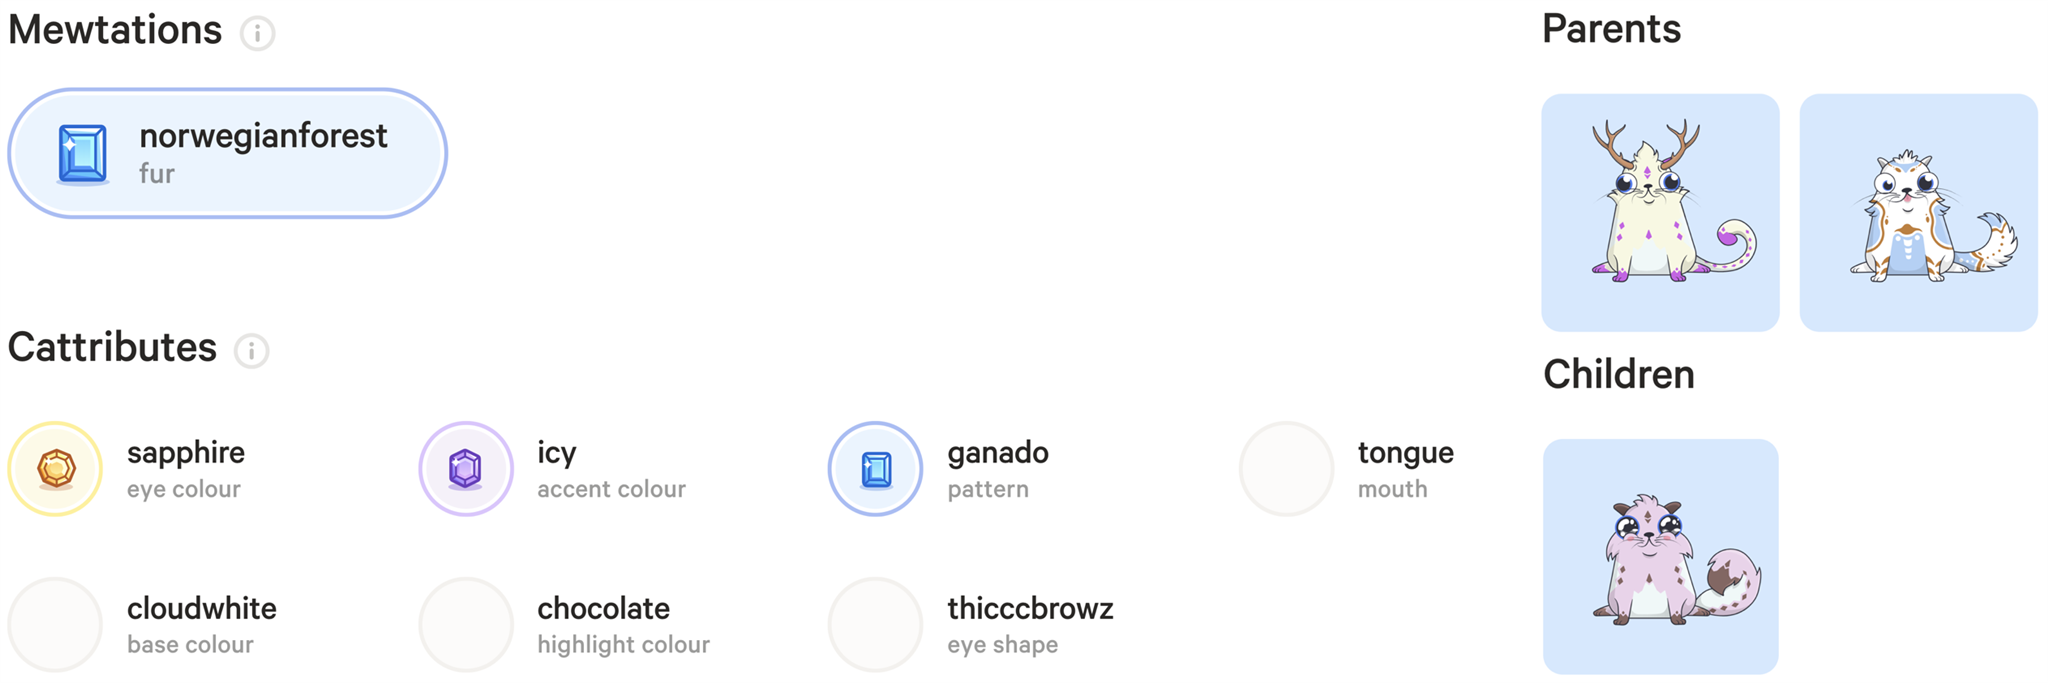
\includegraphics[height=3cm,width=0.9\textwidth]{images/7_implemenation_and_usecases/kittie_attributes.png}
\caption{The unique attributes of a Kitty.}
\label{fig:attributes}
\end{subfigure}
\begin{subfigure}[b]{0.5\textwidth}
\centering

\includegraphics[height=2.8cm]{images/7_implemenation_and_usecases/kittie.png}
\caption{An instance of a Kitty.}
\label{fig:kitty}
\end{subfigure}
\begin{subfigure}[b]{0.5\textwidth}
\centering
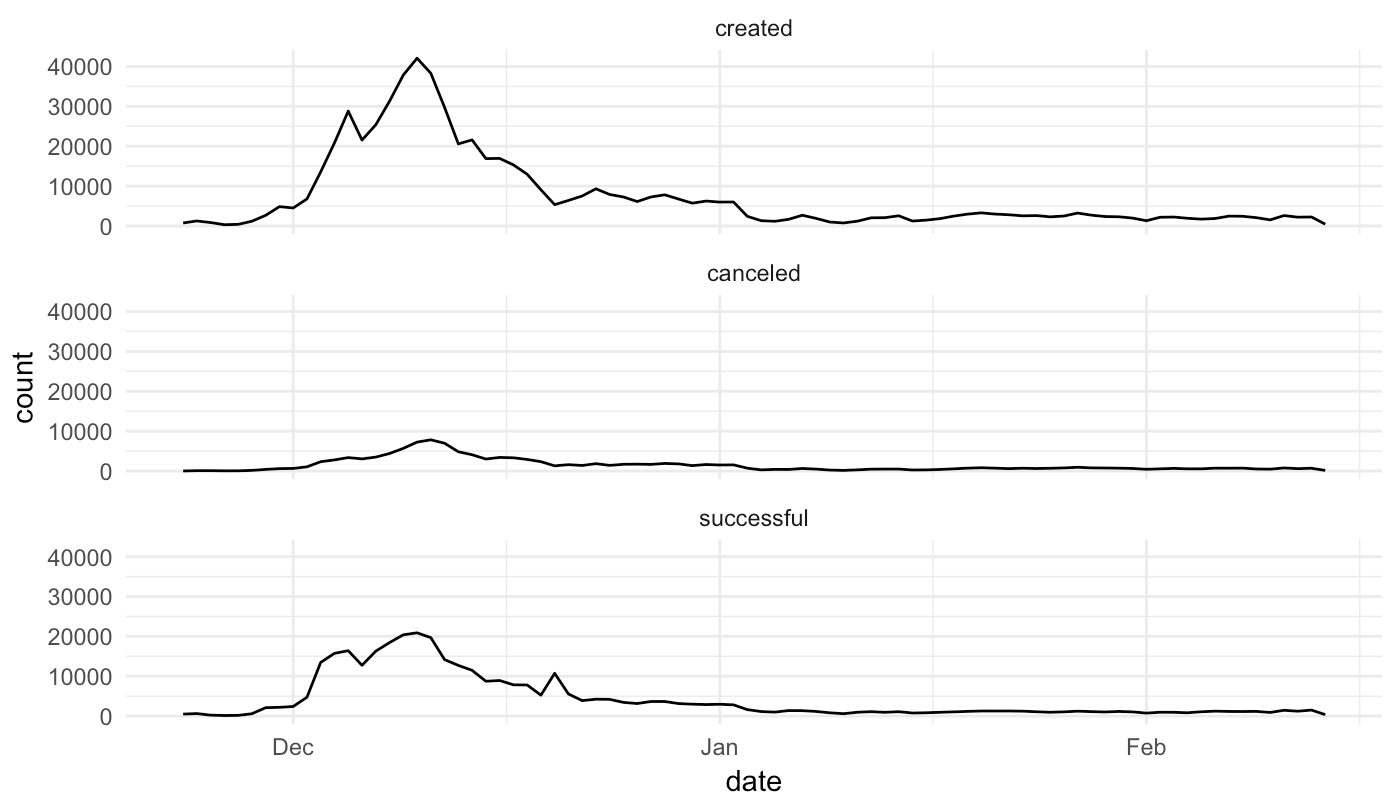
\includegraphics[height=2.8cm,width=\textwidth]{images/7_implemenation_and_usecases/auction_event.png}
\caption{History of three types of auction events.}
\label{fig:auction}
\end{subfigure}
\begin{subfigure}[b]{0.5\textwidth}
\centering
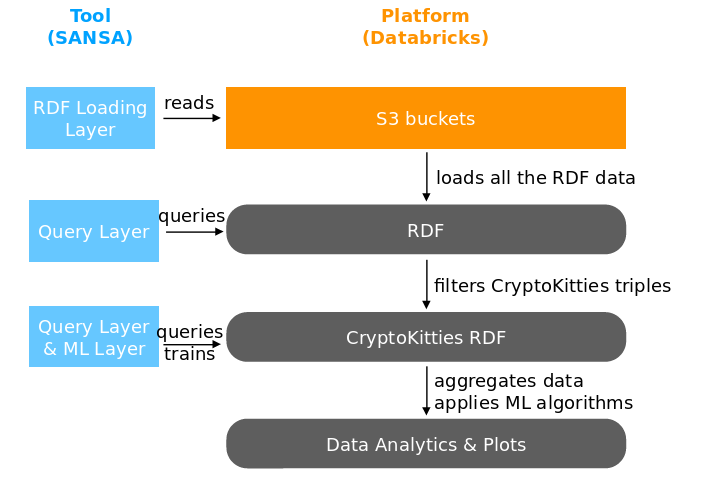
\includegraphics[width=1\textwidth]{images/7_implemenation_and_usecases/CryptoSANSA-pipeline.png}
\caption{The process pipeline.}
\label{fig:pipeline}
\end{subfigure}
\begin{subfigure}[b]{0.5\textwidth}
\centering
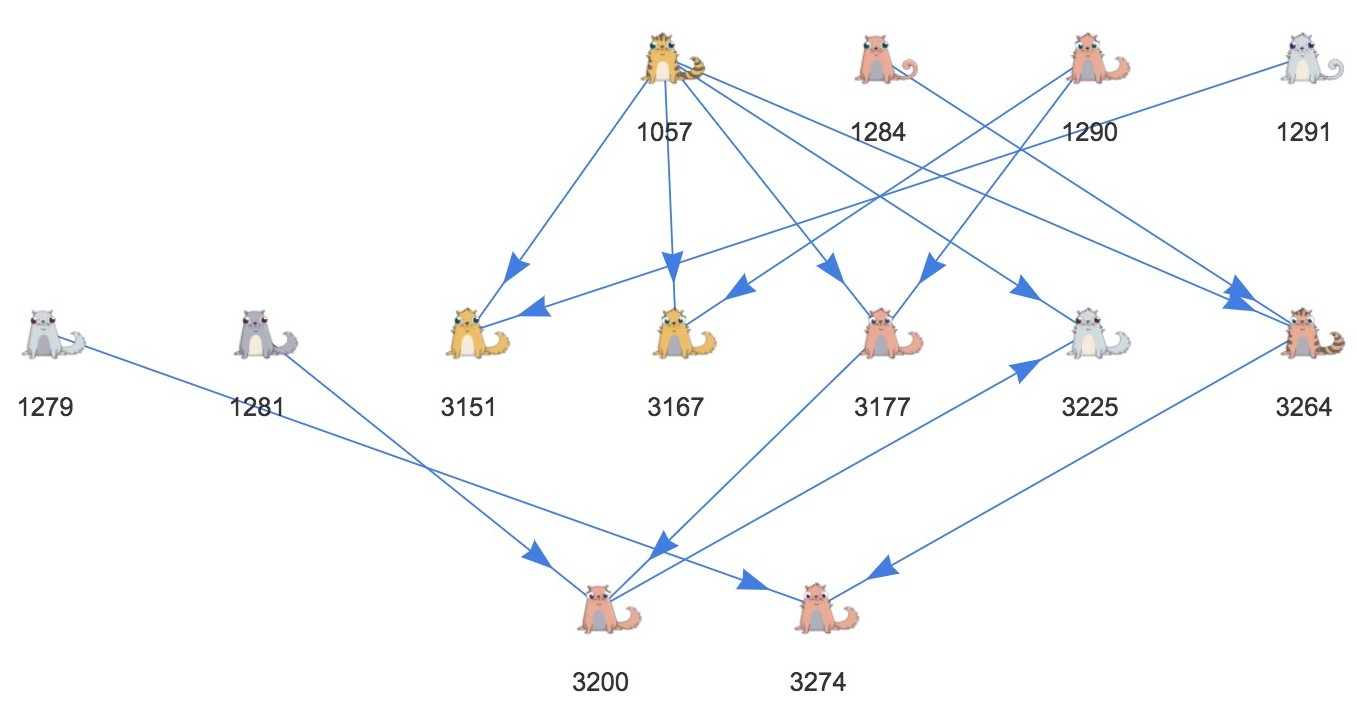
\includegraphics[height=4cm,width=\textwidth]{images/7_implemenation_and_usecases/incest-crop.jpeg}
\caption{An illustration of a small family tree.}
\label{fig:incest}
\end{subfigure}
\caption{\textbf{Leveraging Blockchain RDF Data with SANSA: CryptoKitties as a Use Case}.}
\label{fig:crypto-sansa}
\end{figure*}

\paragraph*{CryptoKitties\footnote{\url{https://www.cryptokitties.co/} (last accessed June 11\textsuperscript{th} 2018 )}} is one of the first games to be built on blockchain technology.
In particular, CryptoKitties initiated and released the first generation virtual kitties, with delicately designed icons and genes sequences. 
All the kitties are virtual with some biological feature settings. 
Shown in Figure~\ref{fig:kitty} is a kitty with its specific biological attributes displayed in Figure~\ref{fig:attributes}. 
The attributes are stored in a sequence, succeeded from its parents' gene sequences, with possibility of \textit{mewtations}.
An owner can sell, breed or gift it to other user.
When users sell or breed it, they will send transactions to the CryptoKitties smart contracts, which will complete the execution of either transferring ownership between users, or generating a new kitty.
Based on that, game users can trade or breed kitties like traditional collectibles, while having the guarantee that the blockchain will track ownership securely. 
Moreover, one can breed two kitties to create a brand-new, genetically unique offspring.

\paragraph*{Data Challenges.}
Alethio has been exploring efficient means of processing large \gls{RDF} data sets. 
SANSA empowers Alethio to read and query the data at scale as described in Figure~\ref{fig:pipeline}. 
Indeed, once the complete \gls{RDF} data set is loaded, SANSA filters it to retain only the CryptoKitties triples --transactions, contract messages and log information-- before performing more specific analyses.

Practically, the challenges tackled with SANSA can be divided into two groups: game performance and customer behaviors. 
The first one focuses on time series metrics: throughput time, the event volume, number of active users and amount of spent Ether, which can jointly estimate the trend of popularity for the game. 
In Figure \ref{fig:auction}, the history of CryptoKitties auctions events shows clearly that there was a peak of traffic in December after the game was launched for around one month. 
By this time series, we can estimate the popularity of the game throughout history.
The second one requires machine learning algorithms to detect correlations between indicators (e.g. to determine whether richer owners have the tendency to collect special/rare kitties which are more expensive). and topology from a network view. In Figure \ref{fig:incest}, we present a small subset of the kitty family tree, where incest happened during the reproduction: kitty 1057 is the secondary-degree relative (grandparent) of kitty 3200, while later it bred with kitty 3200 and gave birth to kitty 3225.


\section{Mining Big Data applications logs using the SANSA framework}
\label{sec:bde-use-case}
Big Data Europe (BDE)\furl{https://github.com/big-data-europe}~\cite{Auer+ICWE-2017} is a large Horizon2020 funded EU project which offers an open source big data processing platform allowing users to install numerous big data processing tools and frameworks. 
The platform has been tested and used by the 17 different partners of the project scattered across Europe and its 7 different use cases cover a variety of societal challenges like climate, health, weather etc.

More specifically, BDE also allows creation of a workflow for a stack containing many applications, each serving a particular data value chain. 
An important feature of the integrator interface is the $\verb|mu.semte.ch|$ micro service which transforms docker events to \gls{RDF} and stores them in a triple store. 
The work is also being done towards storing the network logs in the triple store, by translating the http network traffic as triples as they occur in the network.
This network log data combined with the docker event data grows over time and provides a useful source that can help in analysing the event-call-time proximity. 
SANSA has been used to perform useful analytics over this data and provide a possibility to create user profiles for the BDI platform. 

\subsubsection{Application example: a Smart Green and Integrated Transport}
The H2020 Societal Challenge 4\furl{https://www.big-data-europe.eu/pilot-transport/}, Smart Green and Integrated Transport, covers a broad topic ranging from urban mobility, to safety, logistics, transport system integration, infrastructure monitoring and planning.
\begin{figure*}[h]
\centering
	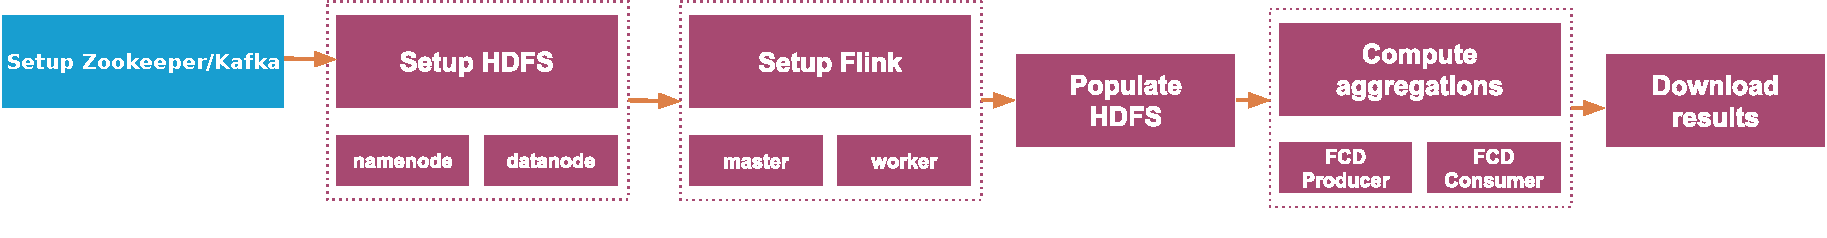
\includegraphics[width=\textwidth]{images/7_implemenation_and_usecases/SC4_Arch.pdf}
	\caption{\textbf{Transport pilot initialization workflow}.
	The SC4 initialization pipeline including different BDE dockerized components.
	}
	\label{fig:SC4-pipeline}
\end{figure*}
Transport systems consume huge flows of data to provide services, monitor infrastructures and discover the usage patterns in order to forecasting what will be the status in the near or distant future. 
All these systems consume streams of data from different sources and in different formats. 
In the SC4 pilot we have therefore decided to build a pilot that can ingest, transform, integrate and store streams of data that have spatial and temporal dimensions. 
One of the project  partner, CERTH-HIT, is managing a system that monitors the traffic flow in Thessaloniki, Greece, using floating car data from a transport company. 
The legacy system is based on a relational database, stored procedures and R scripts to map-match the location of the vehicles to the road segments and compute the traffic flow and average speed among other statistical parameters. 
The result of the computation is used for monitoring and as input for forecasting the value of the parameters in the near future and is made available through a web service. 
The aim of the pilot is to address the scalability issues of the current system leveraging the availability of distributed frameworks and the containerization technology for the deployment of services in different environments.

The pilot is based on the microservices architecture where different software components, producers and consumers, communicate through a messaging system connecting data sources to data sinks.
Producers and consumers are implemented as Flink\furl{http://flink.apache.org/} jobs while Kafka\furl{https://kafka.apache.org/} has been chosen as the messaging system.
The producer fetches the data every two minutes from the web service, stores the records sets into \gls{HDFS}, transforms the records into a binary format, using a schema shared with the consumer, and finally sends the records to a Kafka topic. 
The consumer reads the records from the kafka topic and process them at event time applying the map matching function. 
The consumer must connect to an R server where an R script has been installed to perform the computation for the map matching using the road network data from Open Street Map stored in a PostGis database. 
The consumer adds the identifier of the road segment as an additional field to the original record and finally aggregates the records per road segment and in time windows to compute the traffic flow and the average speed in each road segment. 
The result of the aggregation can be sent to \gls{HDFS} or to Elasticsearch\furl{https://www.elastic.co/products/elasticsearch}. 
From Elasticsearch different visualizations can be created easily with Kibana\furl{https://www.elastic.co/products/kibana}. 
The records with the aggregated values stored in Elasticsearch will be used as input to a forecasting algorithm to predict the traffic flow. 
All the components are available as Docker images and a docker-compose file has been created adding the initialization service and the UI provided by the BDI Stack in order to start the services in the right sequence from the browser (e.g. Zookeeper before Kafka and PostGis and Elasticsearch before the consumer).\furl{https://github.com/big-data-europe/pilot-sc4-fcd-applications}

With such chain of technologies used, it is obvious that many logs are being generated.
BDE uses our approaches for log mining e.g. finding the most frequently errors happening at the specific event.


\section{Scalable Integration of Big POI data using the SANSA framework}
\label{sec:slipo-use-case}

Various organizations like DBpedia~\cite{dbpedia-swj}, Wikidata~\cite{Vrandecic:2014:WFC:2661061.2629489} etc.\ are constantly working for gathering information from different sources and storing it in structured form, e.g.~\gls{RDF}.
\gls{RDF} data allow to model various domains and this characteristic helps to solve problems in different areas i.e., from the medical domain to the geographical domain. 

In this study, we are focusing on \gls{POI}s.
\gls{POI}s are generally characterized by their geospatial coordinates along with their thematic/contextual attributes.
A common \gls{POI} use-case is to find hot zones according to specific topics: i.e. discovering \gls{AOI}s as a result of aggregation of \gls{POI}s.
With the assistance of \gls{AOI}s, one can identify other similar areas in the same or a different city, recognize the distinguishing characteristics of this area, and determine potential types of users (or customers) that would be interested in that area.

In this use case, we propose a flexible architecture to design clustering pipelines for \gls{POI} semantic datasets at once.
Indeed, using large and detailed \gls{RDF} vocabularies allow richer \gls{POI} descriptions.
For example, one \gls{POI} related to a restaurant might be described by its latitude, longitude, food specialty, reviews, address, phone number etc. which could represent up to 50 distinct triples\footnote{\scriptsize See e.g. the SLIPO ontology: \url{https://github.com/SLIPO-EU/poi-data-model/}} leading then to billions of RDF records overall.
As a consequence, we require scalability and build our solution on top of the distributed semantic stack SANSA which benefits from Apache Spark.
The proposed architecture then enables any kind of clustering algorithm combinations on \gls{POI} \gls{RDF} data.

\subsection{Proposed Solution: Architecture Overview}
In order to process RDF (containing POIs) datasets in an efficient and scalable way, we first have to adopt a convenient processing framework.
SANSA is a data-flow engine for distributed computing of large-scale \gls{RDF} datasets. 
It provides \gls{API}s for faster reading, querying, inferencing and apply analytics at scale.
It uses Apache Spark as an underlying engine.
SANSA contains features which are utilized for processing \gls{RDF} data with thematic and spatial information.

\begin{figure*}
    \centering
	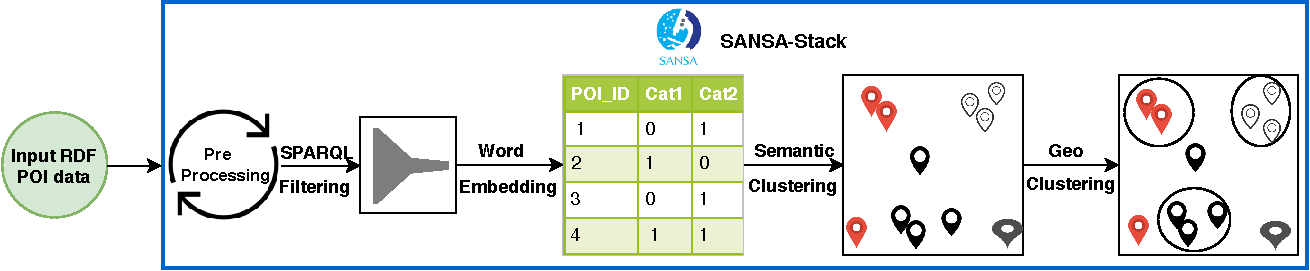
\includegraphics[width=\textwidth]{images/7_implemenation_and_usecases/KmeansPaper8.pdf}
	\caption{\textbf{A Semantic-Geo Clustering flow}.
	It consists of five main components: data pre-processing, SPARQL filtering, word embedding, semantic clustering and geo-clustering.}
	\label{fig:imp-use-case-clustering}
\end{figure*}

Our proposed approach contains up to five main components (which could be enabled/disabled if necessary) namely: data pre-processing, \gls{SPARQL} filtering, word embedding, semantic clustering and geo-clustering.
In particular, in Figure~\ref{fig:imp-use-case-clustering}, we present an example of Semantic-Geospatial clustering pipeline.
Indeed, we consider two types of clustering algorithms: the semantic-based ones and the geo-based ones.

In semantic based clustering algorithms (which do not consider \gls{POI} locations but rather aim at grouping \gls{POI}s according to shared labels), there is a need to transform the \gls{POI}s categorical values to numerical vectors to find the distance between them. 
So far, we can select any word embedding technique among the three available ones namely one-hot encoding, Word2Vec and Multi-Dimensional Scaling.
All the above mentioned methods converts categorical variables into a form that could be provided to semantic clustering algorithms to form groups of non-location-based similarities.

For example, all restaurants are in one cluster whereas all the ATMs in another one.
On the other hand, the geo-clustering methods help to group the spatially closed coordinates with in each semantic cluster.

More generically, our architecture and implementation allow users to design any kind of clustering combinations they would like. Actually, the solution is flexible enough to pipe together more than two clustering ``blocks'' and even to add additional \gls{RDF} datasets into the process after several clustering rounds. In addition, we directly embedded the state-of-the-art clustering algorithms into the SANSA Machine Learning layer\furl{https://github.com/SANSA-Stack/SANSA-ML} so that these pipelines are prone to be built out of the box.


\subsubsection{Application example: a Semantic-Geo clustering pipeline}

To illustrate the feasibility of our approach and demonstrate the potential of the \gls{RDF} \gls{POI} clustering library we developed in SANSA, we present --as an example-- in this section the implementation results of the specific architecture presented in Figure~\ref{fig:imp-use-case-clustering} i.e. a Semantic-Geo clustering pipeline.

In order to test the process and validate the approach, we used an \gls{RDF} \gls{POI} dataset which follows the ontology described in~\cite{Athanasiou2019BigPD} containing around 18\,000 triples which represent information on 623 \gls{POI}s (i.e. around 28 triples per \gls{POI}). We then chose Word2Vec~\cite{mikolov2013distributed} as embedding for the K-means~\cite{kmeans-algo} semantic-clustering algorithm, before running DBSCAN~\cite{ester1996density} as geo-clustering method. In details, we gave the following parameters to the algorithms: 8 clusters within 5 iterations for K-means and $\epsilon=0.002$ with at least 2 points per cluster for DBSCAN.
The complete process took around 20 seconds using a 8GB-memory laptop running a single-node SANSA \& Spark stack.

\begin{figure*}
    \centering
    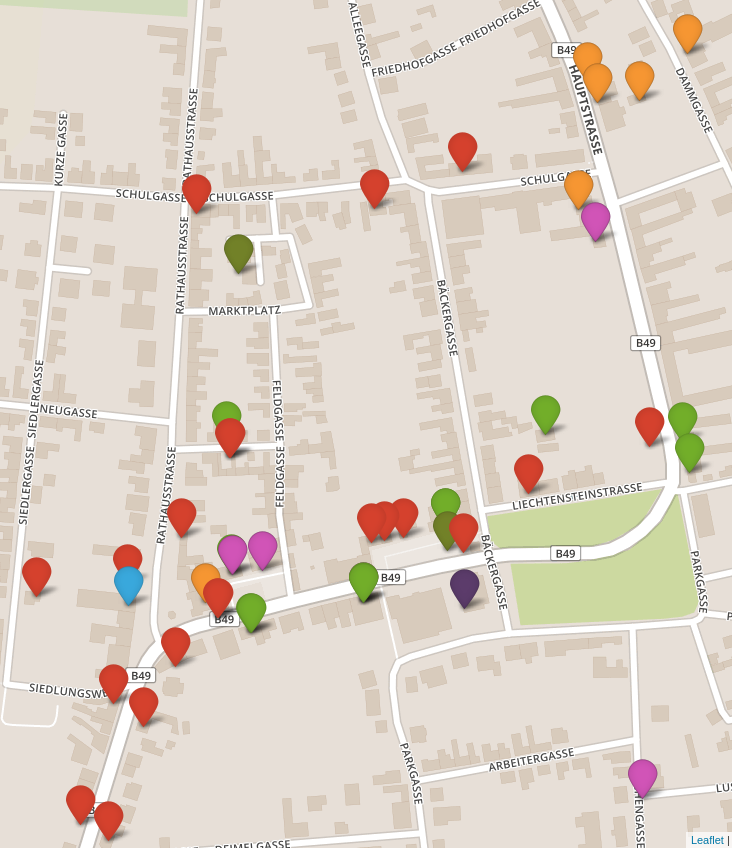
\includegraphics[width=.49\textwidth]{images/7_implemenation_and_usecases/kmean.png}
	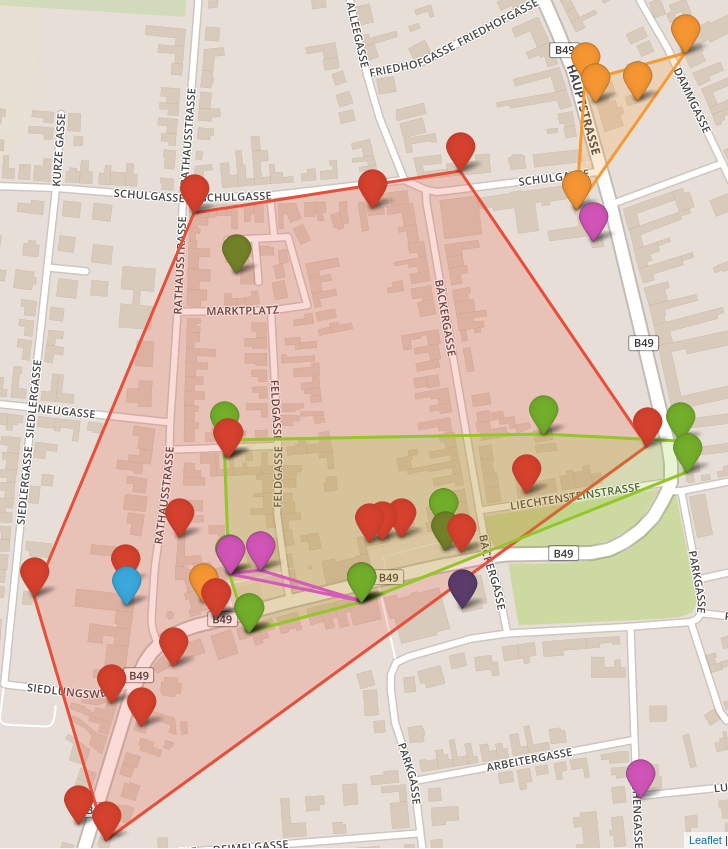
\includegraphics[width=.49\textwidth]{images/7_implemenation_and_usecases/kmeandbscan.png}
    \caption{\textbf{Visualizations (on a map) of the Semantic-Geo clustering pipeline steps}.
    Visualizations of a zoom over a particular Austrian region with K-means results of POIs (left) and geographical clustering with relevant AOIs (right).}
    \label{fig:imp-use-cases-map}
\end{figure*}

We present the results obtained at the various steps in Figure~\ref{fig:imp-use-cases-map} on a map, the figure presents a zoom over a particular Austrian region. 
The figure is twofold, we first display (left side) the only result of the K-means where \gls{POI}s are pinned on a map and where each color corresponds to a specific cluster. 
As expected, the semantic clusters are distributed over the entire country since \gls{POI}s of a color are sharing common ``sense'' with regards to the categories in the ontology. 
As a consequence, the geographical step of aggregation allows then to break those country-spread clusters into pieces and obtain (right side of Figure~\ref{fig:imp-use-cases-map}) relevant \gls{AOI}s. 
In particular, four \gls{AOI}s are visible: an orange one in the corner, a large red one which also embeds a green one and a little magenta.


\section{Summary}
SANSA provides a scalable solution for reading and querying large scale \gls{RDF} data, providing compatibility with machine learning libraries on Spark including GraphX as a graph processing library.

With conventional graph analysis tools, we successfully identified Hubs and Authorities in the Ethereum transaction network and discovered that they are mainly related to exchange wallet and mining pool activities.

This pipeline also provides a possibility to filter out top accounts, which are likely to be exchanges' deposit wallets. 
Furthermore, with the filtered top rank accounts, the ``mixing'' patterns of exchanges' deposit wallets become recognizable. 
This can be a promising tool for detecting previously unknown exchange wallets and lead to a deeper understanding of their behavior patterns for future analyses.
Alethio is investigating DistQualityAssesment as well, for performing large-scale batch quality checks, e.g.~analysing the quality while merging new data, computing attack pattern frequencies and fraud detection. 
Alethio uses our approaches on a cluster of 100 worker nodes to assess the quality of their $\approx$20B\furl{https://linkeddata.aleth.io/} of RDF data.

In addition, we presented a solution to extract \gls{AOI}s from big POI data while considering several dimensions at the same time. The architecture is embedded inside a state-of-the-art Semantic Web stack (i.e.~SANSA) and then benefits from the advantages of it. For instance, it allows source aggregation or datasets filtering via \gls{SPARQL} to only focus on some interesting regions, e.g., a specific country can be selected. 
Moreover, even if we restricted our description in this study to a Semantic-Geo clustering pipeline, our architecture allows any kind of clustering combinations.
Finally, the above-presented pipeline is also openly available from a demonstrating notebook\furl{https://github.com/SANSA-Stack/SANSA-Notebooks} on the SANSA repository.
